\documentclass[11pt, notitlepage]{report}

\usepackage[margin=2cm]{geometry}
\usepackage{amsmath}
\usepackage{graphicx}

\newcommand{\BigO}[1]{\ensuremath{\operatorname{O}\bigl(#1\bigr)}}

\DeclareGraphicsExtensions{.png}

\setlength{\parindent}{0cm}

\title{Randomised Algorithms CW1}
\date{}
\author{Owen Davies \and Charlie Hothersall}

\begin{document}

\maketitle

\section*{Introduction}

In this report we will examine the performance of our implementation of the Skip List, Bloom Filter and Random BInary Search Tree data structures. We will compare the average execution time and the number of comparisons performed for the insert, search and delete operations. The graphs drawn show the performance of the data structures averaged out over 500 repetitions.

\section*{Insertion}

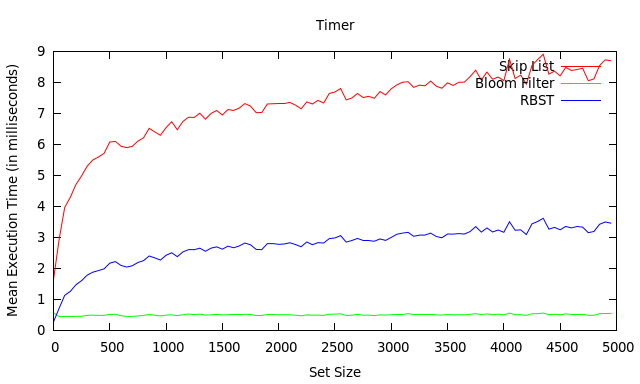
\includegraphics[width=\linewidth]{img/Timer-Add}

Here, the Bloom Filter lives up to it's impressive insertion time of \BigO{k}, with the time being constant (dictated by the 2 hash functions in the implementation) for any set size.\\

The RBST performs very well also, with the mean execution time staying very low even for a large set size. We can see that the line matches a $\log$ n graph exactly - our implementation matches the the theoretical prediction of \BigO{\log n} (where n in the set size).\\


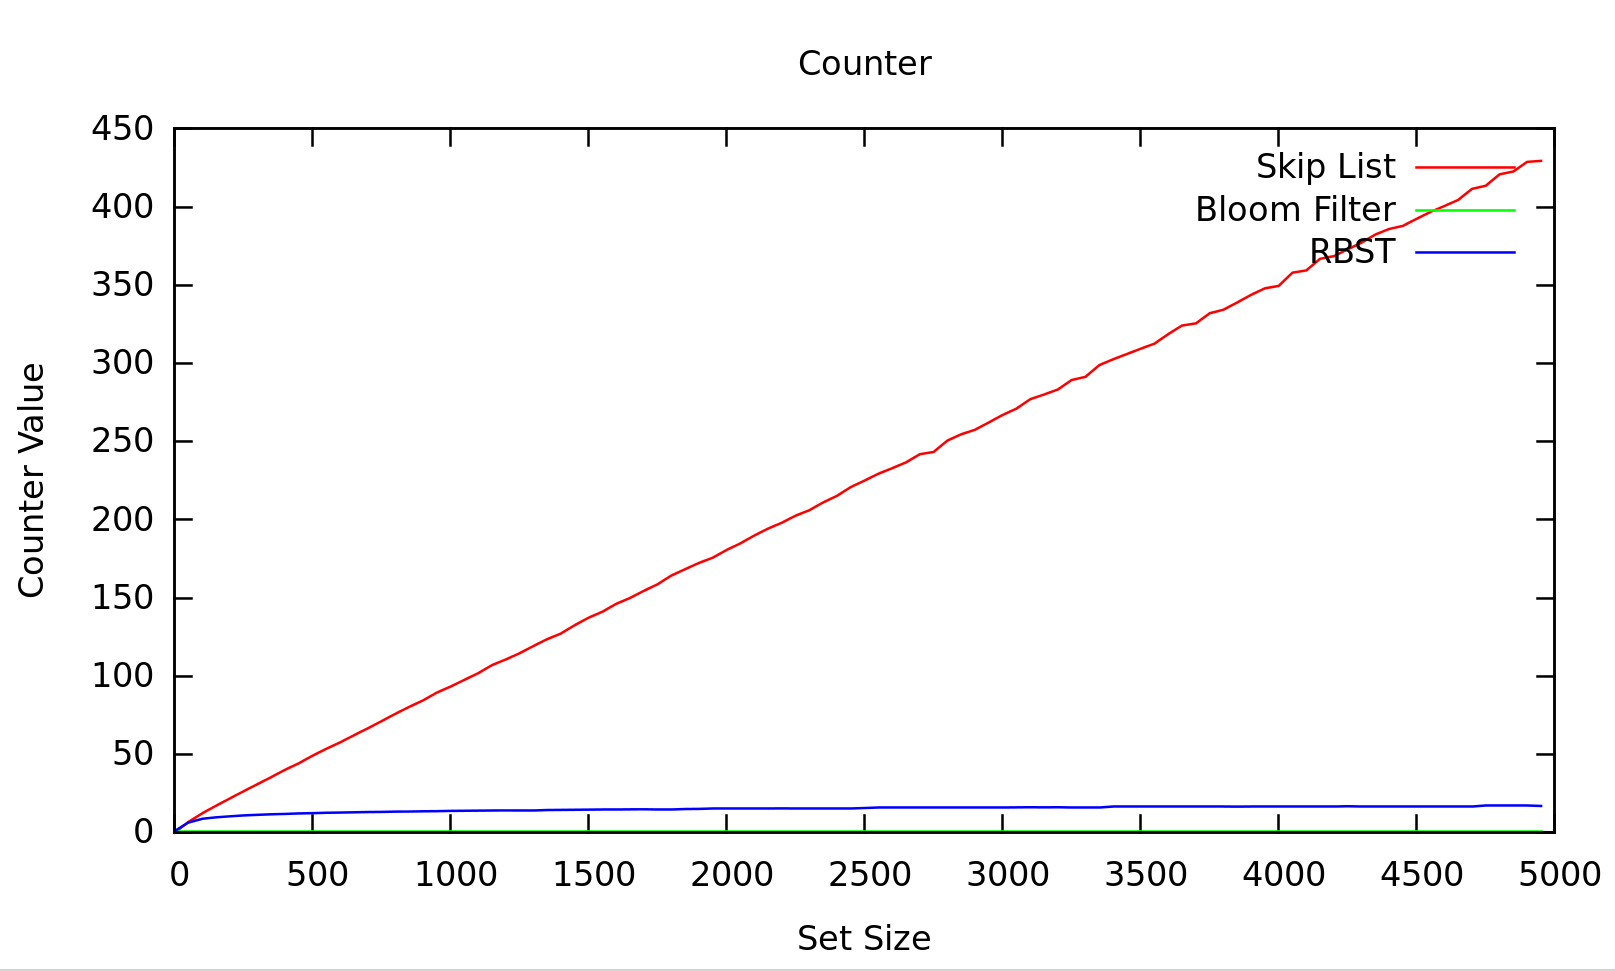
\includegraphics[width=\linewidth]{img/Counter-Add}

The same can be said for the number of comparisons as was said for the execution time. The Bloom Filter is constant for all set sizes as the only computation done is to hash the key and change the correct bits in the filter.\\

The number of comparisons perfomed for RBST insert increases as expected; the bigger the size of the tree, the more recursive calls have to be made. This line still very much conforms to the theoretical complexity of $\log$ n, which makes perfect sense considering the shape of a BST.

\section*{Deletion}

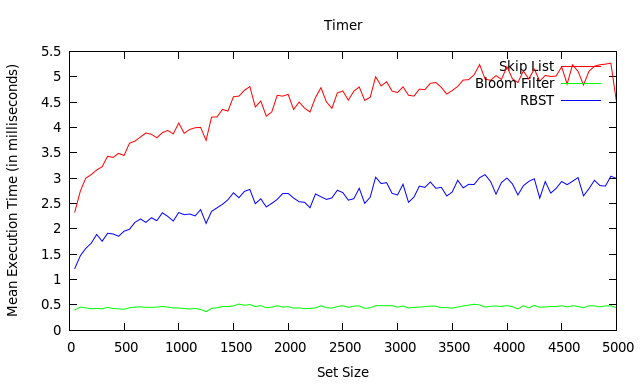
\includegraphics[width=\linewidth]{img/Timer-Del}
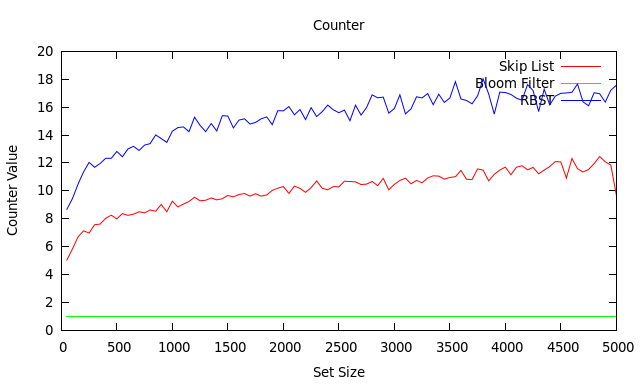
\includegraphics[width=\linewidth]{img/Counter-Del}

\section*{Search}

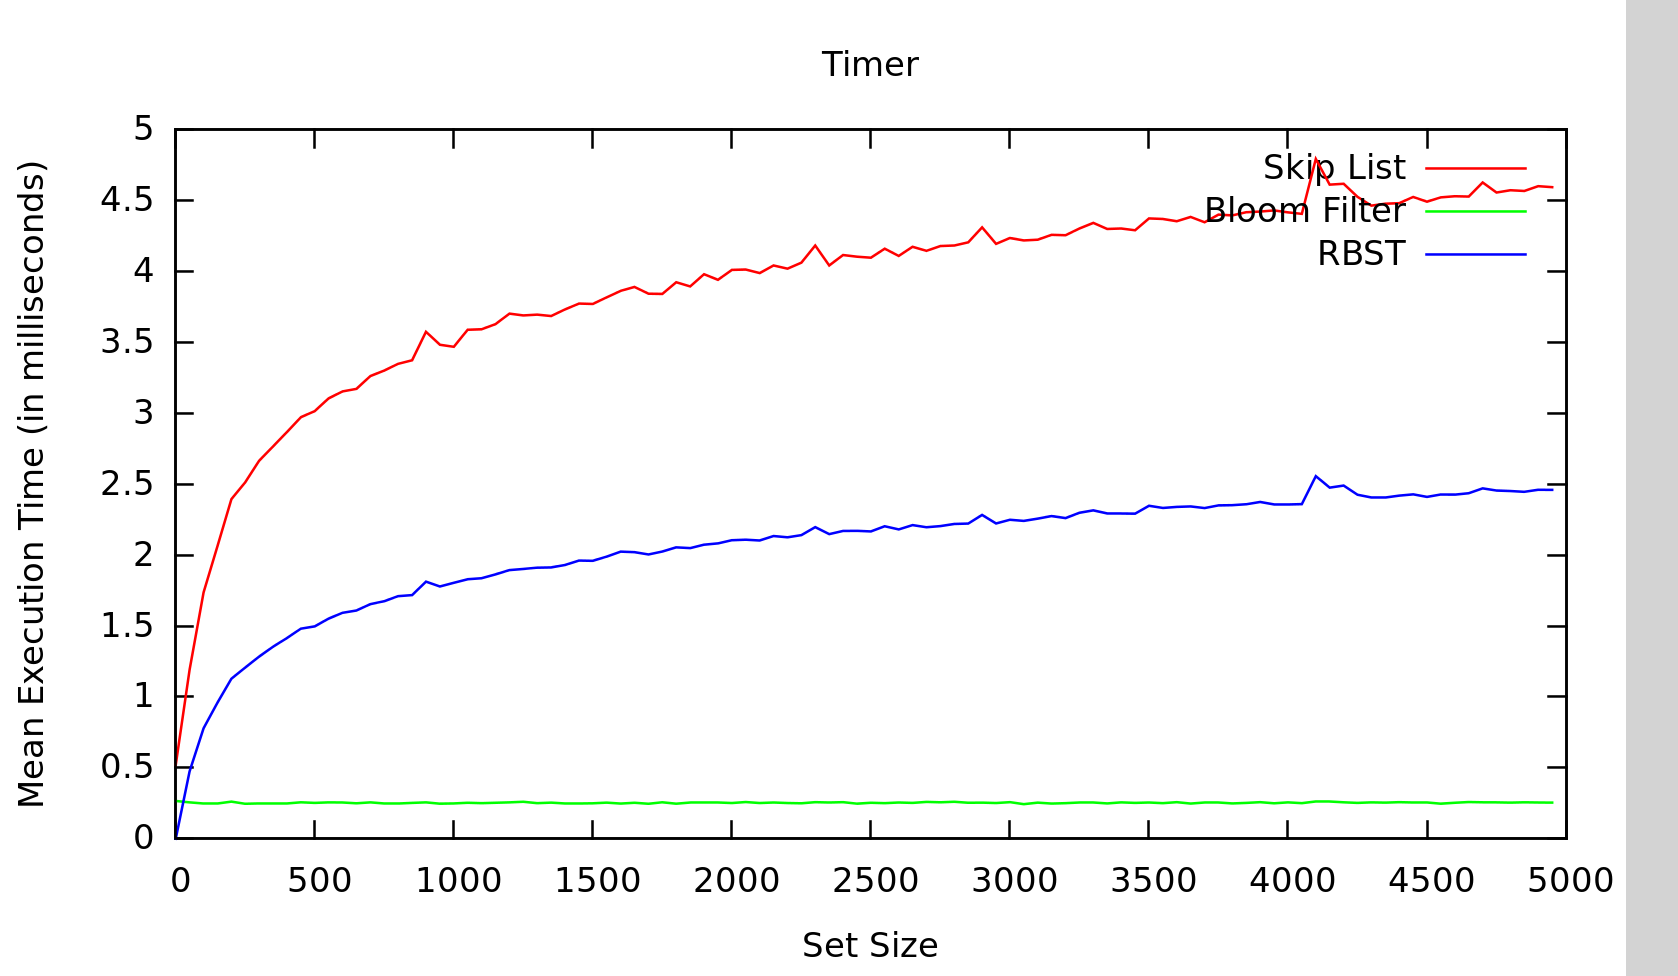
\includegraphics[width=\linewidth]{img/Timer-Find}
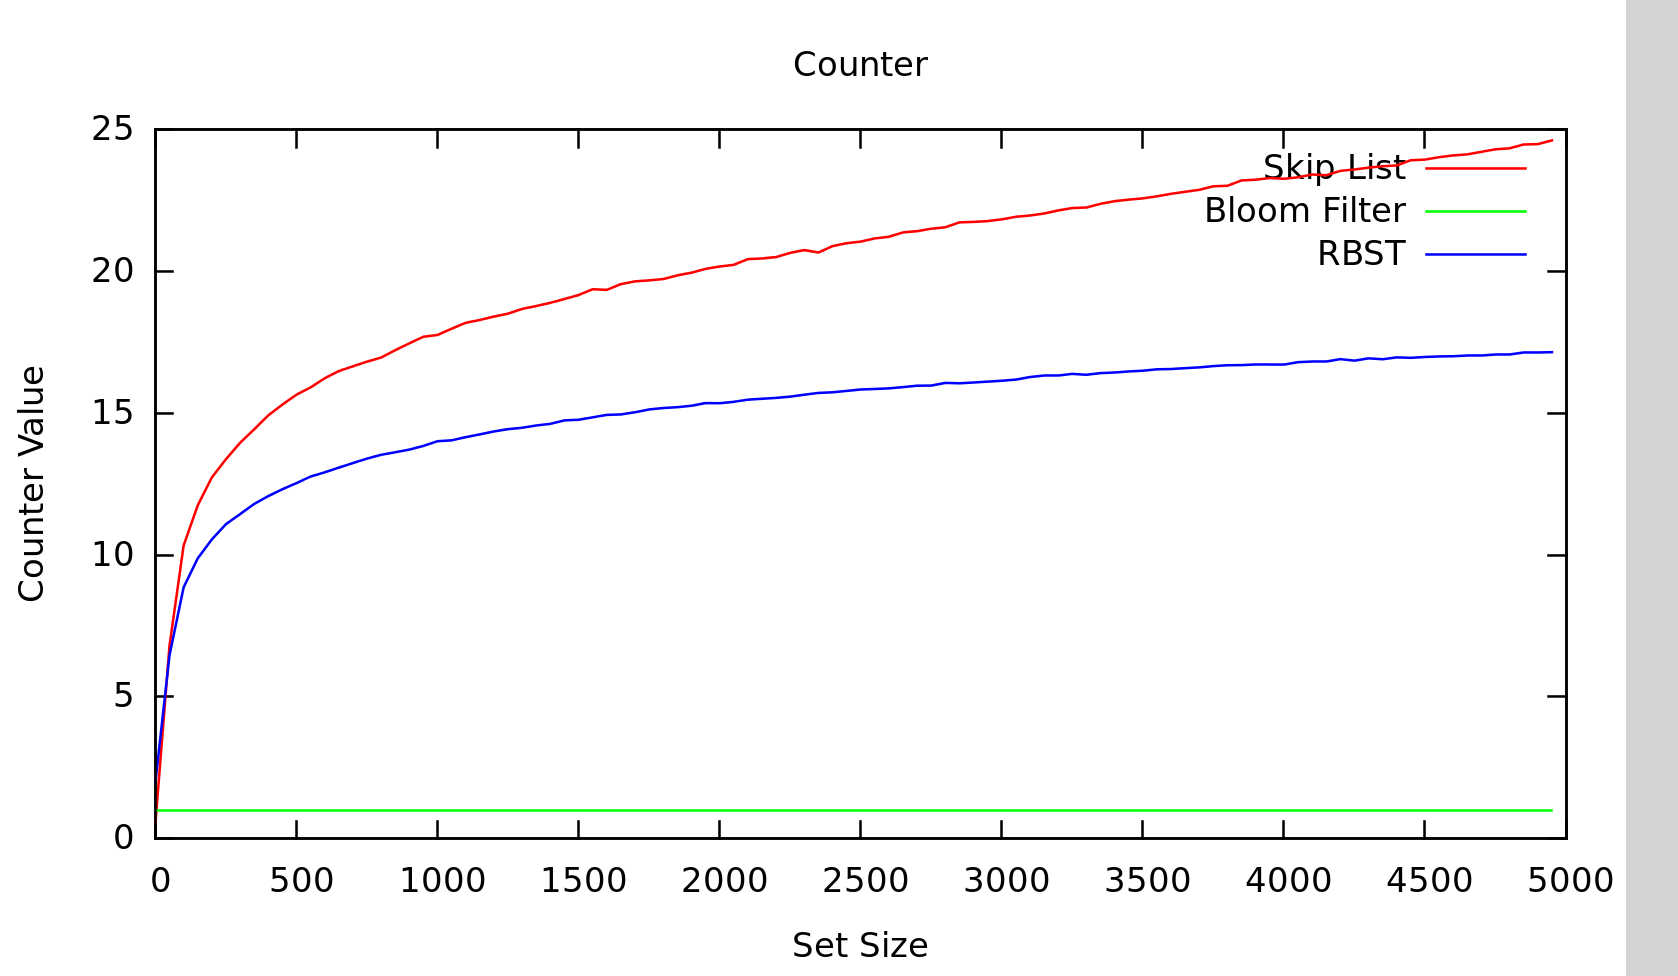
\includegraphics[width=\linewidth]{img/Counter-Find}

\end{document}
